\documentclass[10pt, a4paper]{article}
\usepackage[utf8]{inputenc}
\usepackage{graphicx}
\usepackage[nil, spanish]{babel}

\begin{document}
  \begin{titlepage}
    \begin{center}
        \vspace*{1cm}
            
        \Huge
        \textbf{Análisis matemático I.}
            
        \vspace{0.5cm}
        \LARGE
        Resumen de teoremas, demostraciones y conceptos.
            
        \vspace{1.5cm}
            
        % \textbf{CORRADI, Joaquín I. - 2225513}\\
            
        \vfill
            
        \vspace{0.8cm}
            
        % 
\includegraphics[width=0.2\textwidth]{logoucc.png}
            
        \Large
        CORRADI, Joaquín I.
        Universidad Católica de Córdoba\\
            
    \end{center}
\end{titlepage}


  \section*{Consignas del trabajo}

    \begin{enumerate}

      \item \begin{enumerate}

        \item Luego de leer el texto \textit{"Historicidad"}, especificamente lo
          referido a las tres temporalidades, ejemplificar cada una de las temporalidades
          con letras de canciones.

        \item Justificar.

      \end{enumerate}

      \item \begin{enumerate}

        \item ¿Cuál es la crítica de Gevaert al concepto de \textit{"determinismo"}?

        \item El autor describe los factores que justifican la ilusión determinista; 
          señalar un ejemplo, presente en la vida cotidiana contemporánea, para cada 
          uno de estos factores y justificar las relaciones.

      \end{enumerate}

      \item Completar un cuadro, teniendo en cuenta lo planteado por 
        el texto \textit{"Historicidad"} respecto al pasado, presente y futuro.

  \end{enumerate}

  \vspace{1.5cm}

  \section*{Resolución de consignas}
    
    \begin{enumerate}

      \item \begin{enumerate}
          \item La temporalidad restaurador se puede relacionar con la canción 
            \textit{"Stressed Out"} de \textit{Twenty One Pilots}, la temporalidad constructor 
            se puede relacionar con la canción \textit{"Good Days"} de 
            \textit{SZA}, y la temporaliad utópico se puede relacionar 
            con la canción \textit{"The Man"} de \textit{Taylor Swift}.
        \item En el caso de la primer temporalidad el autor señala que añora los
          tiempos pasados cuando era niño, resalta que todo era más sencillos y
          mejor, y lo deja claro con la siguiente frase del estribillo:
          \textit{wish we could turn back time to the good old days} lo que se 
          traduce como \textit{ojalá pudiéramos hacer retroceder el tiempo a 
          los buenos viejos tiempos}.\\
          Las canción relacionada con la segunda temporalidad se habla de la 
          importancia de dejar ir el pasado y seguir adelante hacia un futuro 
          mejor luego de una ruptura amorosa, pero también se remarca el 
          valor del presente y en encontrar la felicidad en el momento actual.\\
          Finalmente la última canción que se relaciona con la temporalidad utópica
          habla sobre que hay que actuar con un propósito y tener metas y 
          objetivos claros. La cantante habla sobre cómo ella es 
          vista por algunos como una revolucionaria ya que imagina un mundo 
          sin desigualdad,
          pero ella se ve a sí  misma como alguien que simplemente está luchando 
          por lo que cree que es correcto y lo que piensa es un futuro ideal.
      \end{enumerate} 

      \item \begin{enumerate}

        \item El autor critica la idea de \textit{"determinismo"} porque cree que 
          puede limitar a las personas. Él argumenta que pensar que todo en la 
          vida está predeterminado y que no tenemos control sobre nuestro destino 
          puede hacernos sentir indefensos. \\

          Asimismo, señala que el determinismo puede tener un impacto negativo en 
          la creatividad y la innovación, al no dejar espacio para la libre elección 
          y la imaginación. También destaca que puede tener implicaciones éticas 
          y morales problemáticas, al librarse de responsabilidad personal en 
          las decisiones y acciones.\\

          Desde la perspectiva del autor, el determinismo es una visión simplista 
          de la realidad,  y él, en cambio, apoya una visión más realista.

        \item Los factores que determinan la ilusión determinista son los siguientes:\\ 
          lusión retrospectiva. A menudo pensamos que los eventos pasados eran 
          inevitables porque ya sucedieron y no se pueden cambiar. Por ejemplo, 
          la caída del Muro de Berlín en 1989 se debe a tensiones políticas y 
          económicas que se habían estado gestando en Europa del Este durante 
          mucho tiempo. Esta idea puede surgir porque no podemos cambiar el 
          pasado.\\

          Impotencia frente a los acontecimientos. A veces sentimos que no podemos
          cambiar eventos importantes de la historia, como el cambio 
          climático. Aunque intentemos hacer algo al respecto, parece que estos 
          eventos van a suceder de todas maneras, como si estuvieran destinados 
          a ocurrir.\\ 

          Deseo de ofrecer una base ideológica a un compromiso histórico. Hay personas 
          que creen en el determinismo histórico para justificar su lucha o 
          compromiso histórico. El marxismo es un ejemplo de esta idea, ya que 
          sostiene que la historia se desarrolla a través de las luchas de clases 
          y hacia la victoria del proletariado. Para el comunismo, esta idea es 
          importante porque la libertad individual podría poner en peligro la 
          teoría marxista y su visión de la sociedad perfecta.\\
          
          Creencia en el mandamiento divino. Algunas personas creen que Dios 
          ha planeado todo lo que sucede en la historia y que los eventos ocurren 
          de una manera específica. Esto puede hacer que piensen que los humanos 
          no tienen mucho control sobre lo que sucede y que los desastres naturales 
          y los conflictos armados son parte del plan de Dios y no pueden ser cambiados. 
      \end{enumerate}
        
    \item 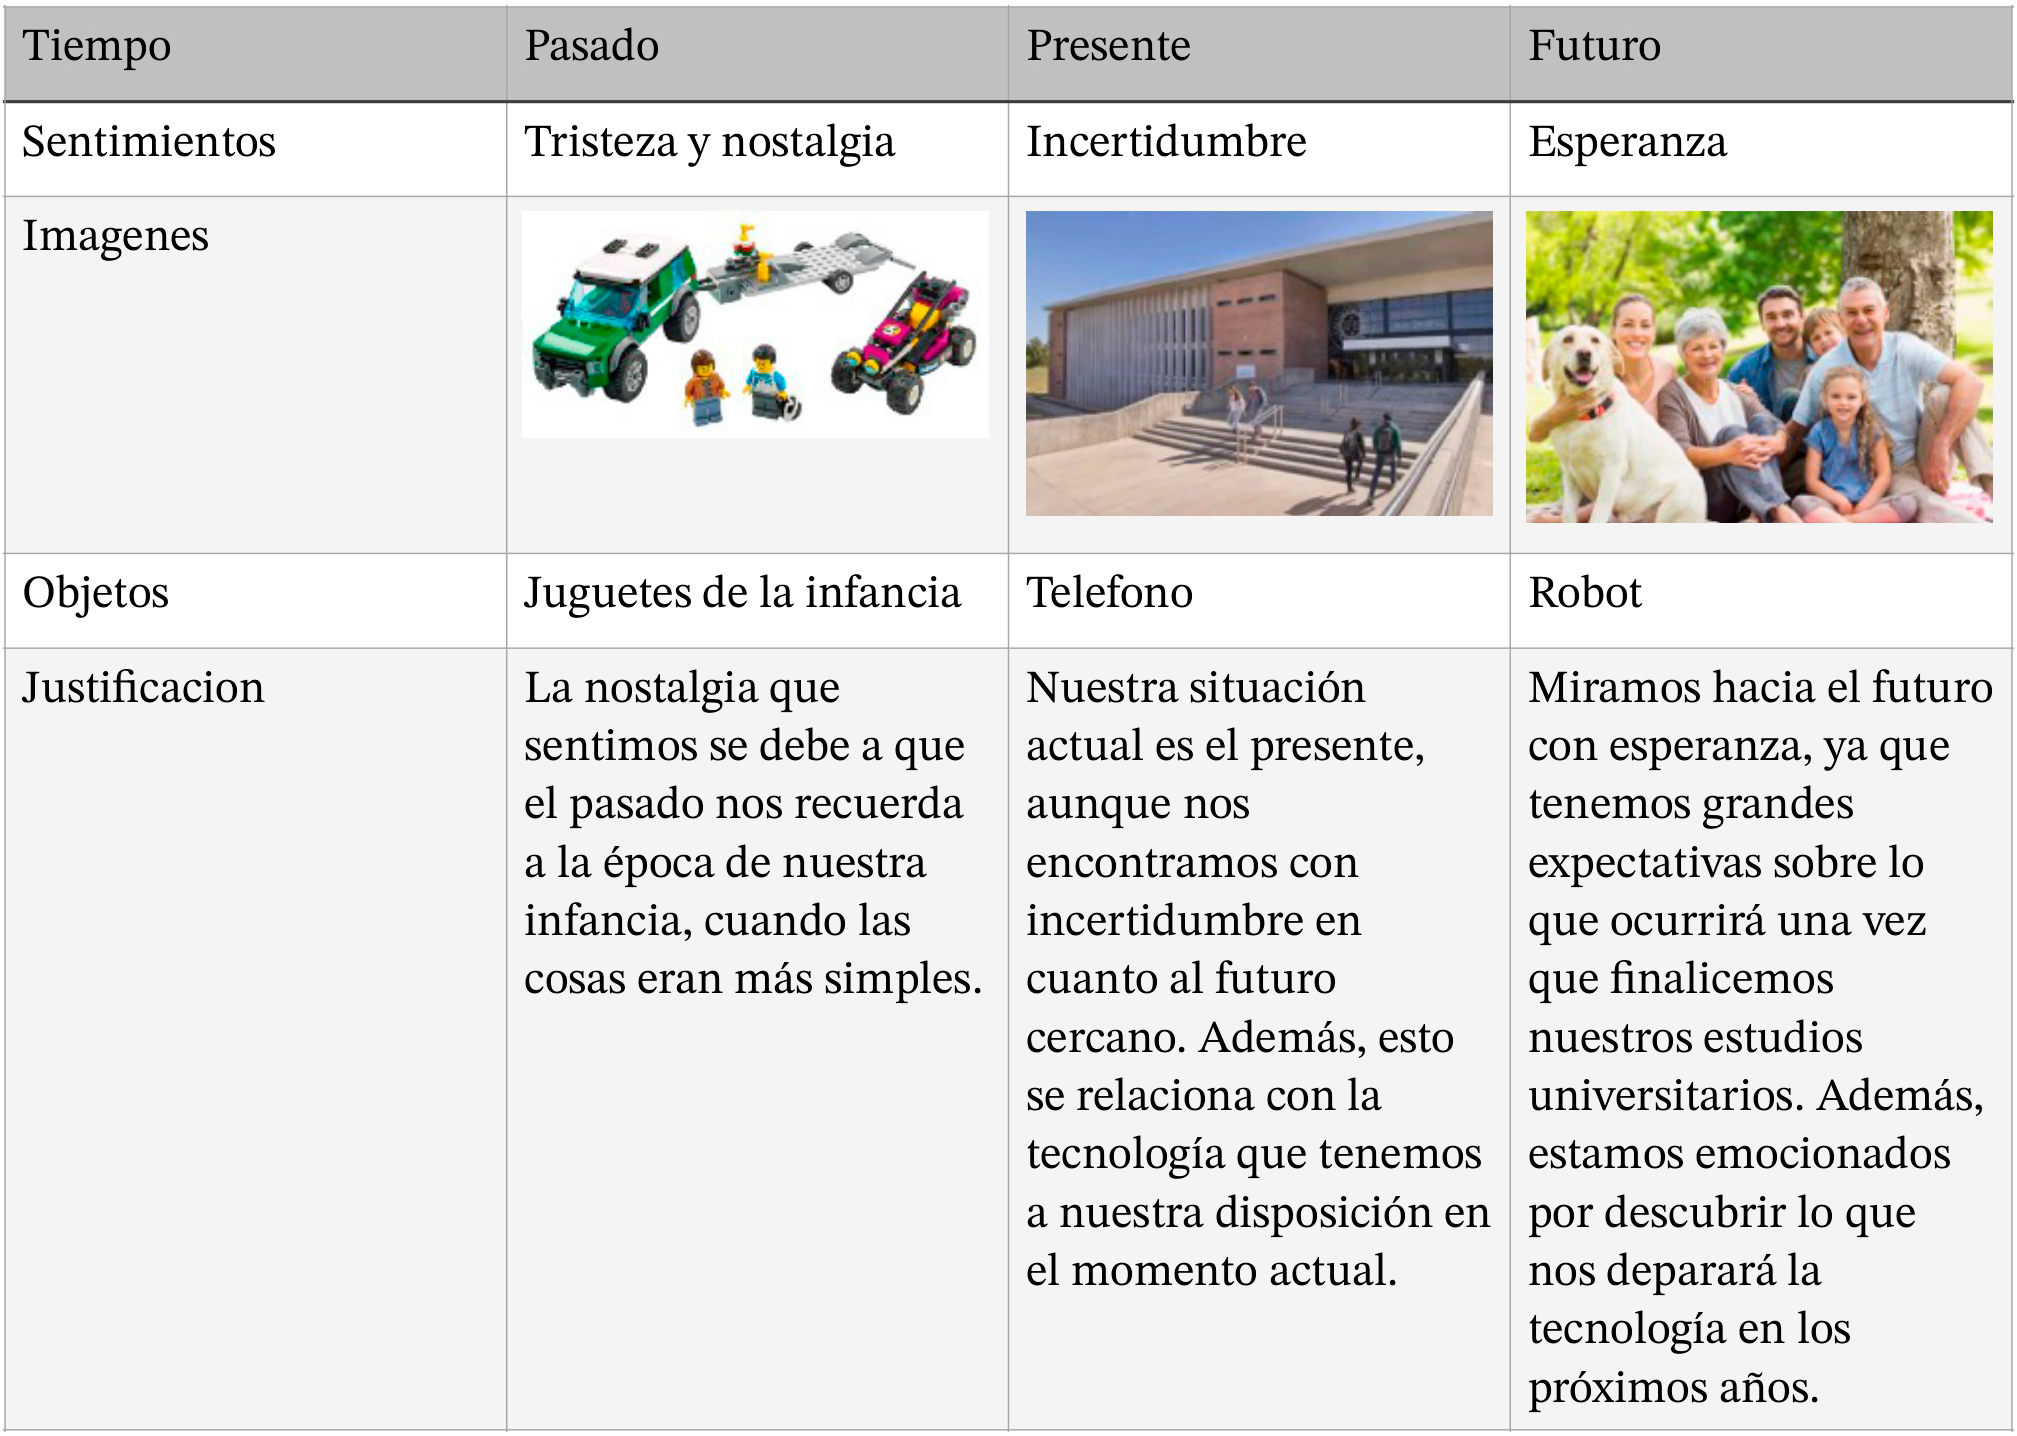
\includegraphics[width=1\textwidth]{cuadro.jpg}
        
    \end{enumerate}
    
\end{document}
